\section{Evaluation}
We deployed and evaluated N2O on a local high end cluster. Two representative applications cap3, ImageMagick were chosen for testing. As we focus on reduction in completion time of jobs, the overheads of N2O must be measured at first. Also the computing resource usage was considered and compared. Then we have a discussion about threshold tuning in N2O system.

\subsection{setup}

The local cluster we used is a production one in Tsinghua University, which has hundreds of  server nodes. While each node has tens of GBs of RAM and two Intel Xeon X5670 2.93 GHz CPUs, each CPU has 6 cores. InfiniBand network and LUSTRE parallel file system are deployed in the cluster. With Load Sharing Facility (LSF) job scheduling system, Hundreds of Java Virtual Machines (JVMs) are launched as a LSF job in the cluster. These JVMs are added as compute nodes in ProActive Resource Manager. We used the cluster just in this way, adding the cluster as a LSF node source to the ProActive Resource Manager.

We evaluated N2O on two hand-picked applications. Cap3 is a well known Expressed Sequence Tag (EST) sequence assembly program in bioinformatics, and ImageMagick is also a classic open source picture processing tool. In the cap3 case, there are many EST sequence files in FASTA format. So it is naturally splitted, with a XML descriptor template we provided, it is simple to parallel the job. Gaussian blur is a filter of ImageMagick blurring an image by a Gaussian function to reduce image noise. It is a widely used effect in graphics software, also known as Gaussian smoothing. In this case, the job is rendering a huge size image with Gaussian blur filter, the image was cut into small pieces with ImageMagick first, then filtered , join together at last. 

We use two metrics for evaluation: job completion time and computing resource usage. As a job consists of lots of tasks, which may run in parallel, the job completion time refers to the duration of job submitted and all tasks of the job finished. We use the average rate of successful jobs completion in a fixed period, as a system metric. Considering speculative executions call for extra computing resource, we measure the computing resource usage with CPU utilization statistics, monitoring by ProActive Resource Manager. Given the baseline and N2O CPU utilization with same workflows, the cost of speculative executions can be calculated.

 We deployed N2O as a speculative execution module in ProActive Scheduler. ProActive Scheduler is a high level job scheduling system base on ProActive library. With ProActive Resource Manager, which can combine lots of infrastructures, jobs and workflows can be submitted and scheduled to use a variety of computing resources by ProActive Scheduler. A job is described with a XML descriptor in details.

\subsection{Is outlier exist ?}

As a high end cluster, each server node has powerful CPU, sufficient memory, and enhanced with the InfiniBand network and high performance parallel file system. The heterogenity of hardware is little. Is outliers will come out in a short several minutes execution ?

We randomly select some server nodes as a node source, and submit a job with lots of cap3 executions with same input data on hundreds of JVM nodes. Then we change the node source to some other random server nodes, and do the same. We choose different period of day to repeat the same test. We found that even in a several minutes execution, sometimes there are some outliers in different server nodes and different time unfortunately.

\begin{figure*}
\centering
\subfigure[In the Afternoon] {
  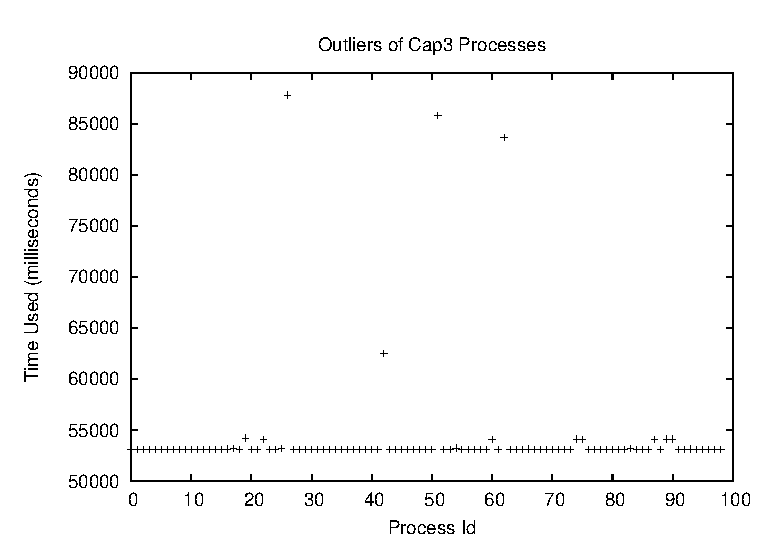
\includegraphics[width=0.45\textwidth]{figures/outliers.eps}
}
\subfigure[In the Midnight] {
  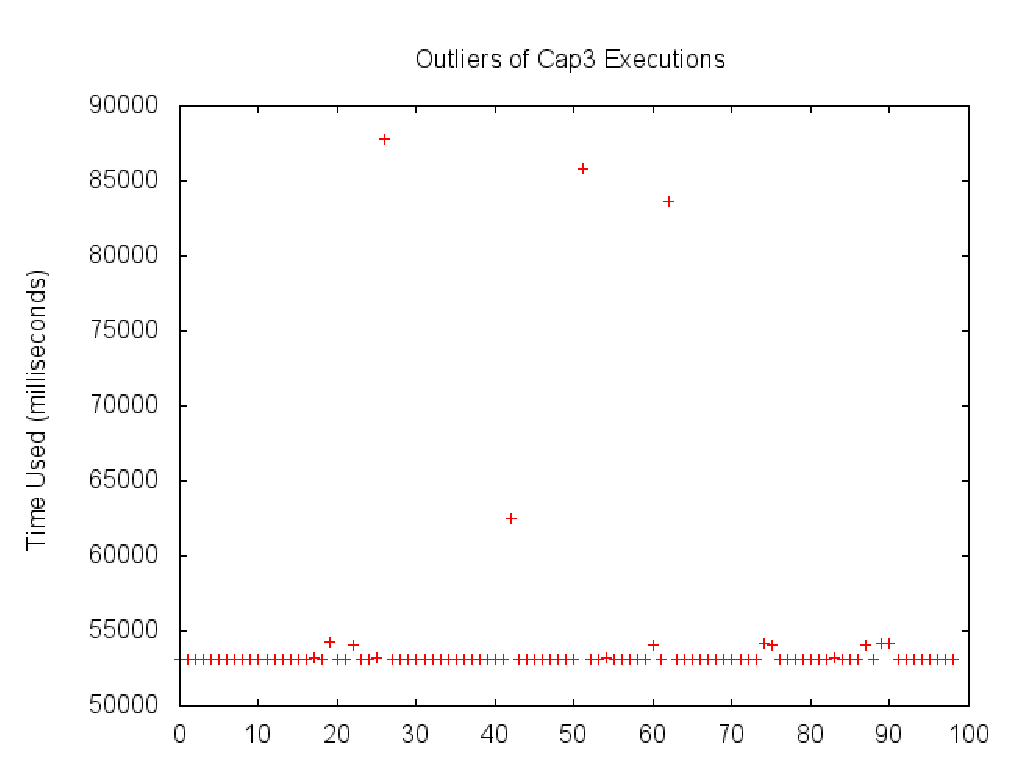
\includegraphics[width=0.45\textwidth]{figures/yaoutliers.eps}
}
\caption{Scatter of Cap3 Execution Time with Random 100 Nodes in Cluster}
\label{figure:outlier}
\end{figure*}

We pick up two pieces of this experiment, and make a scatter plots Figure 0. As shown in this figure, (a) has much more outlier than (b), and outliers need nearly twice or more time to complete the same task. As one server node contains several JVM nodes, The physical outliers is not as much as outliers of JVM nodes. With this naive inspection, we can conclude that even in high end clusters, there are a small number of outliers in some server nodes which may just work busily and some period of day when lots of jobs in the cluster.

\subsection{Overheads and Accuracy of Instrumentation}

Binary instrumentation often cost a very high overhead, which may tens of  times slow than no instrumentation executions. Although static binary instrumentation is more efficiency than dynamic ones, a few percent to tens of percent overhead of tracing all function entries, shown in the Figure 1 (a) and (b), can not be put up with production clusters. 

To evaluate our trace approach with samples, we run the cap3 and ImageMagick in one server node of the high end cluster. Each application is tested tens of times with different inputs. Figure 1 shows the results of this experiment, On average, instrumentation with all function entries costs 8\% ~ 11\% extra time to complete the execution, while instrumentation with sampling used in N2O needs only 0.03\% ~ 0.1\% extra time costs.

\begin{figure*}
\centering
\subfigure[Cap3] {
  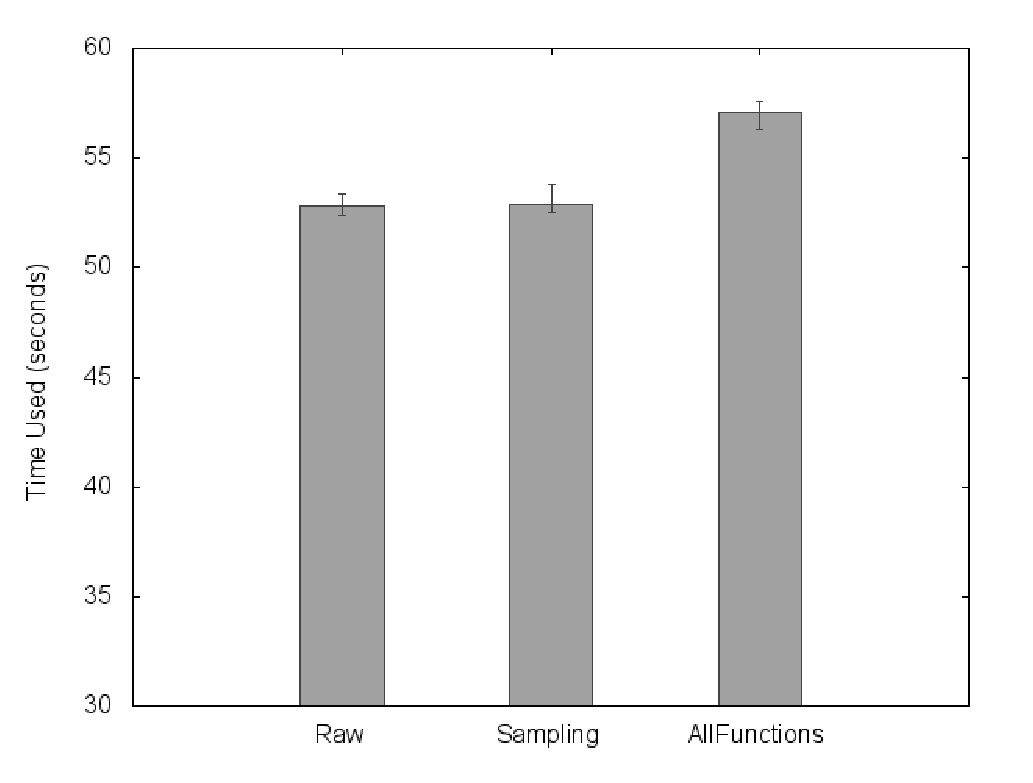
\includegraphics[width=0.45\textwidth]{figures/overhead_cap3.eps}
}
\subfigure[GaussianBlur] {
  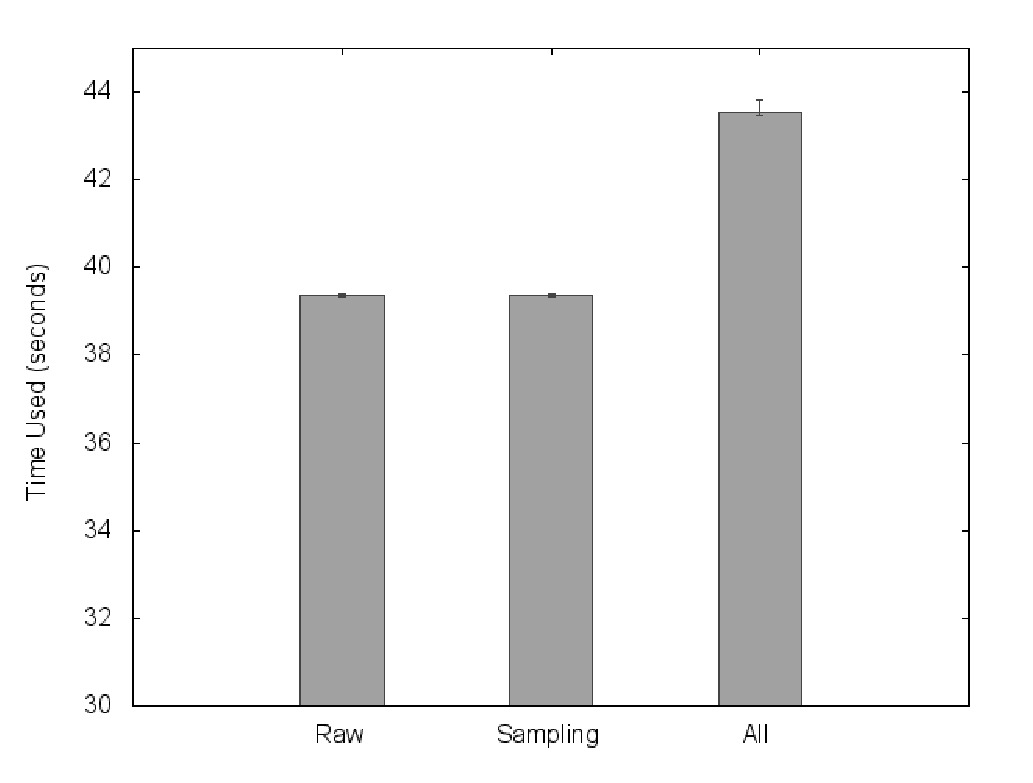
\includegraphics[width=0.45\textwidth]{figures/overhead_gaussianblur.eps}
}
\caption{Overheads of Instrumentation}
\label{figure:overheads}
\end{figure*}

Such low overheads make N2O is enough efficient to deployed in a production system. But samples can not cover all executions, means the instrumentation way based on samples may sometime mistake parts of tracepoint caused progress report inaccurate. So we make a inspection with some trace cases of executions of cap3 and ImageMagick. We noticed that the progress trace with instrumentations with all function entries is more smooth than those with samples, such as ImageMagick execution cases shown in Figure 2. But in some cases the samples way is a little smooth than instrumentation with all functions, such as Cap3 case shown in Figure 2.

\begin{figure}
\centering
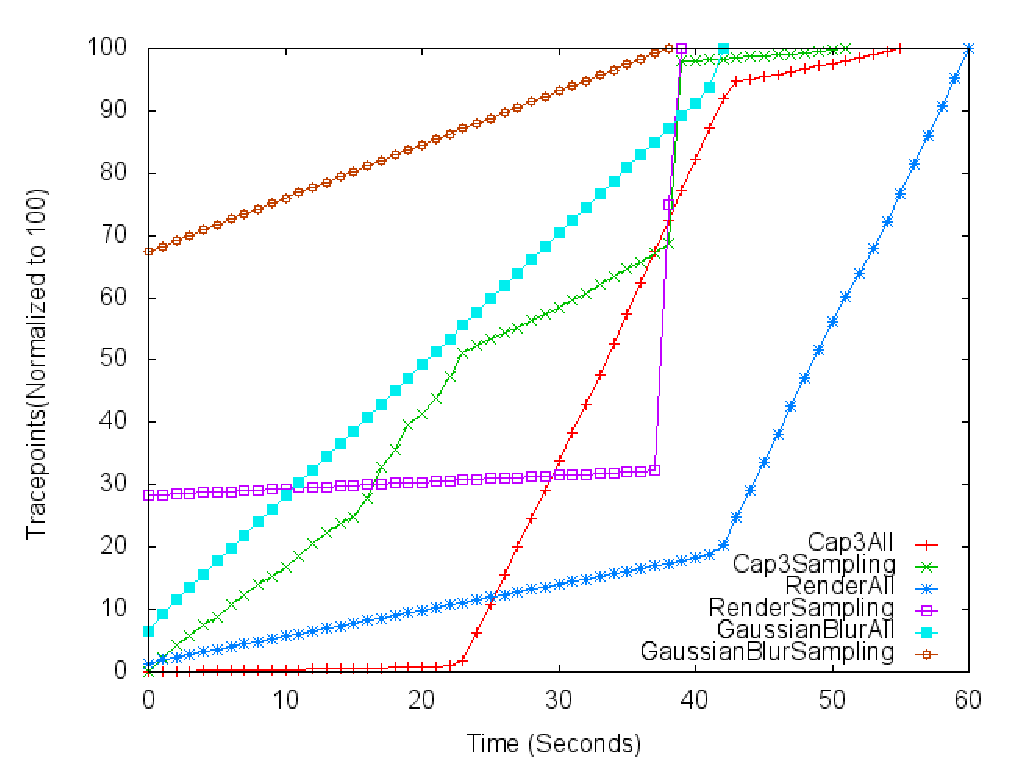
\includegraphics[width=0.9\columnwidth]{figures/tracepoints_all_vs_sampling.eps}
\caption{Tracepoints' Trends}
\label{figure:tracepoints}
\end{figure}

Since each execution is arbitrary with different inputs and conditions completely, every function may last short and long time slots in different executions. Unfortunately, we can not make an inference of absolute execution progress with  trace of instrumentation all function entries. Even instrumentation with all basic binary blocks or with all cpu instructions, there is no absolutely precision as no two identical leaves in the world. 

But a relative smooth tracepoints hit rate can be guaranteed with instrumentation in same granularity, as shown in Figure 2, each line is composed  of few smooth segments. The outliers detection approach we proposed is inspired by this inspection. We use the relative progress to catch the outliers, so the way instrumentation with samplings is enough to us.

\subsection{Can N2O mitigate outliers ?}

Reduction in job completion time is a critical metric. We submitted Cap3 and Gaussian Blur jobs fifty times each to PA Scheduler with and without N2O. Figure 3 (a) and Figure 3 (b) show that job completion time improve by roughly 25\% on average. The histogram plots the best, worst, average reduction of Cap3 jobs and Gaussian Blur jobs. In the worst case of Cap3, there is a little increment of job completion with N2O, caused by a worst choose in speculative execution. On average, the reduction of job completion time with N2O is significant. Without N2O, caused of the hinder of outliers, the completion time of jobs has a big deviation with the best case, However with N2O, the completion time of jobs declined towards to the best case. These two experiments show that N2O mitigate the outliers efficiently.

\begin{figure*}
\centering
\subfigure[Cap3] {
  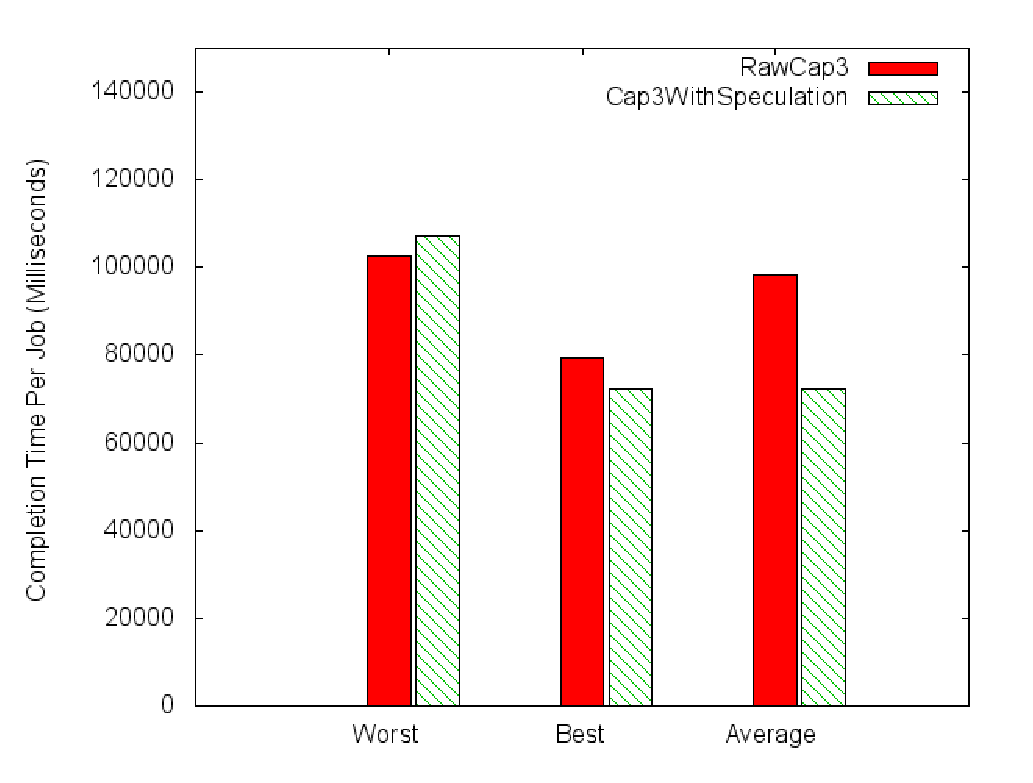
\includegraphics[width=0.45\textwidth]{figures/completiontime_cap3.eps}
}
\subfigure[GaussianBlur] {
  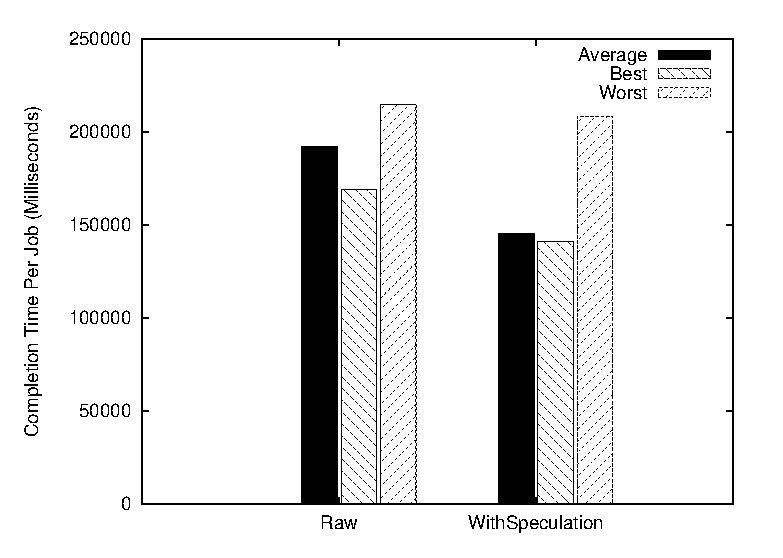
\includegraphics[width=0.45\textwidth]{figures/completiontime_gaussianblur.eps}
}
\caption{Job Completion Time}
\label{figure:completiontime}
\end{figure*}

N2O can bring benefit to job schedulers with improvement of job completion time. At the same time, It needs some amount of computing resource in addition. In aforementioned test, We collected the statistics data of CPU usage from ProActive Resource Manager and plotted a histogram as follows.

\begin{figure}
\centering
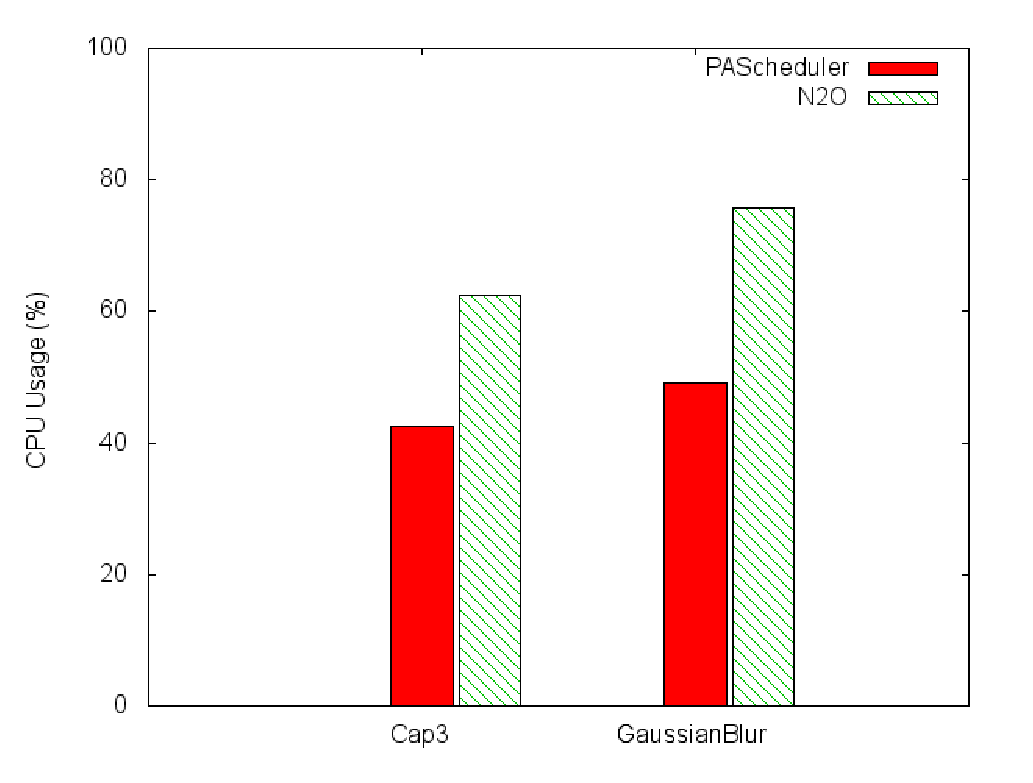
\includegraphics[width=0.9\columnwidth]{figures/resource_usage.eps}
\caption{Computing Resource Usage}
\label{figure:resourceusage}
\end{figure}

As shown in Figure 5, 20\% ~ 30\% more computing resource has been used by N2O for speculative executions. This make sense for some local clusters, which has low utilization and throughput. N2O helps them scheduling jobs more efficiency, and more computing resources used means the reduce of server idle time. But for a busy cluster or a cloud environment, where computing resource is not free, we expect speculative executions use resource as little as possible. We will analysis how to reduce waste of computing resource with little loss of reduction of the job completion time, and for some error-prone environment N2O can even use less computing resource with less failure executions.

\subsection{Discussion}

How slow will outliers mostly be? Or when how much one execution is behind the majority, it must be an outlier? The threshold of outliers is critical for N2O. In our outlier detection approach, we use a naive one-degree Kmeans Clustering algorithm, and we use the variation of the centers of clusters to judge if one of them contains outliers. When the coefficient of variation is larger than threshold T, N2O see that clustering of executions as outliers.

\begin{figure}
\centering
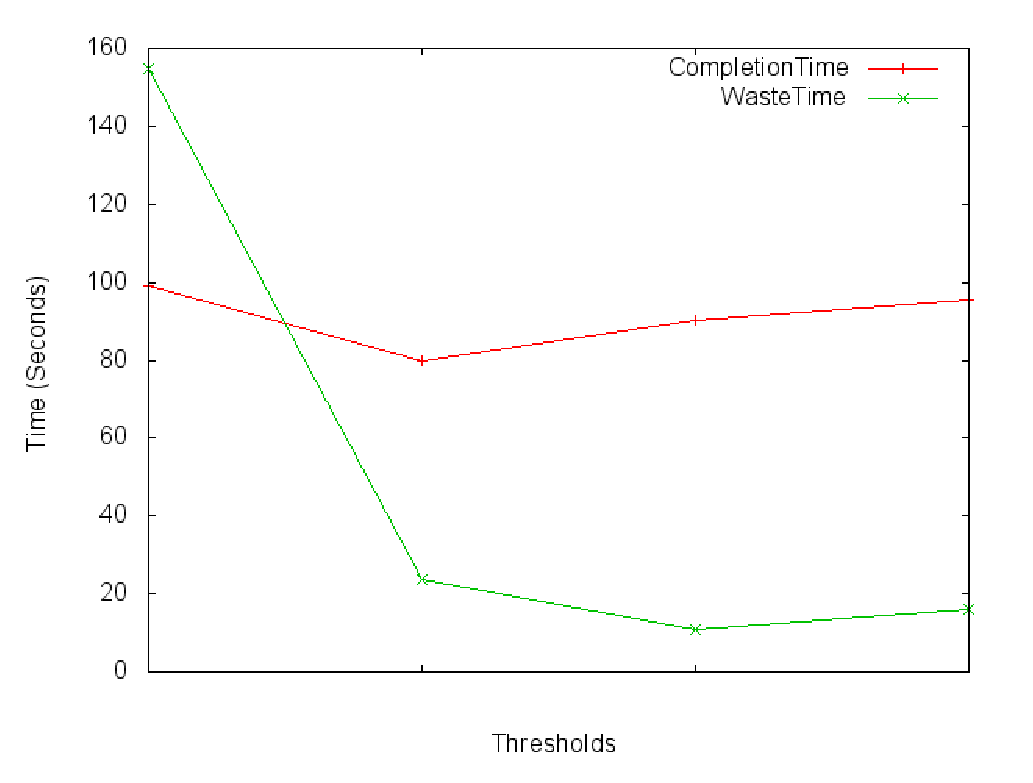
\includegraphics[width=0.9\columnwidth]{figures/threshold&completiontime.eps}
\caption{Completion Time / Waste Time with Threshold Tuning}
\label{figure:thresholdtuning}
\end{figure}

We use a fix server node running a shell script costing lots of CPU as the fake outlier. And make sure others nodes are running normally, if some unexpected outliers found, we just drop the execution result. In this way, we make sure of the other variation little. Tuning the threshold T from low to high, we run a Cap3 job which was splitted into 100 parallel executions to see the sensitivity. In Figure 6, As threshold rise, waste execution time declined and keeps low, completion time declined first and  turn up at a pivot. When threshold still increase, N2O finds little outliers and becomes lag to response. 

\begin{figure}
\centering
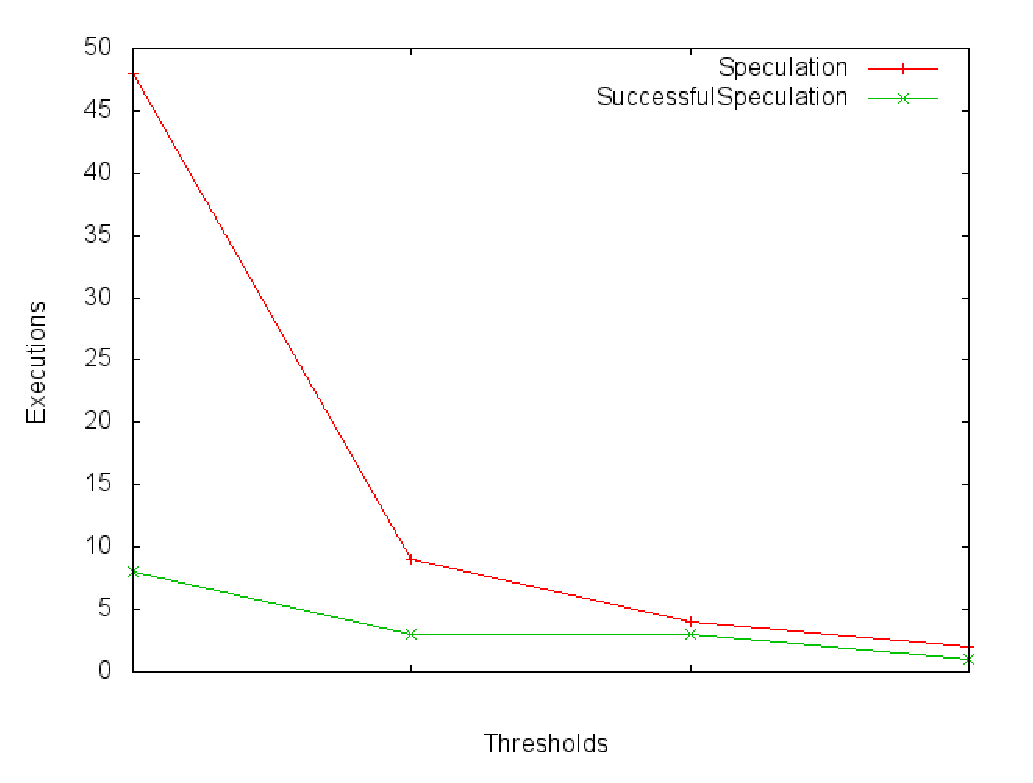
\includegraphics[width=0.9\columnwidth]{figures/threshold&speculation.eps}
\caption{Speculations / Successful Speculations with Threshold Tuning}
\label{figure:yetanotherthresholdtuning}
\end{figure}

A low threshold may be false positive, and cause a large mounts of speculative executions. These has been shown in Figure 7, which means a low success rate of speculations and wasting a lot of computing resource. With a meaningful threshold mitigate the false positive risks and keeps sensitive with outliers, this is the critical for N2O.
